

\section{深さ優先探索}

この節では平面性判定を解決する線形時間アルゴリズムを設計するために、
基本的な枠組みである深さ優先探索について考察する。
また、深さ優先探索の応用として
グラフの$2$-辺連結性を線形時間で判定するアルゴリズムを与える。






%%%%%%%%%%%%%%%%%%%%%%%%%%%%%%%%%%%%%%%%%%%%%%%%%%%%%%%%%%%%%%%%%%%%% 深さ優先探索
\subsection{深さ優先探索の基本原理}
%平面性判定に入る前に、軽く$2$-辺連結性判定に触れておく。
%グラフが$2$-辺連結であるかどうかは橋の有無で判定できる。
%橋はそれを除去すると連結成分の個数を1つ増やす辺である。
%橋検出は深さ優先探索で$O(n+m)$時間で解決することができる。
%$n,~m$はそれぞれ頂点と辺の個数。
%\vspace*{-0.7\intextsep}
\setcolumnwidth{0.75\textwidth, 0.25\textwidth}
\begin{paracol}{2}

深さ優先探索は、任意の頂点から探索を開始し、
まだ訪問していない頂点$v$を発見したら直ちに$v$に遷移し、
新たに$v$の隣接頂点の中から未訪問の頂点を見つけようとする探索方法である。
ただし、すべての隣接頂点が訪問済みならまだ調べ終わっていない頂点まで
戻って探索を再開する。
探索を開始する頂点を根と呼ぶ。

\paragraph{深さ優先探索木}
対象のグラフの各辺は頂点遷移に従い向き付けされ、
根と今調べている頂点の間には常に有向パスが存在することが保証できる。
このとき頂点発見に貢献した辺の集まりが誘導する部分グラフは有向木となる。
この有向木を深さ優先探索木と呼ぶ。
深さ優先探索木を構成する辺を木辺、それ以外の念のため調べてみたが既に発見済みの頂点だった
辺を補木辺という。
%補木辺という呼称は、対象グラフ$G=(V, E)$が連結である場合DFS木は全域木であり、
%木辺と補木辺の集合は$E$の集合分割となる。
%このとき補木辺の集合は、木辺集合の補集合として参照できることから採っている。


\switchcolumn
\vspace{-2.\intextsep}
\begin{figure}[ht]
\centering
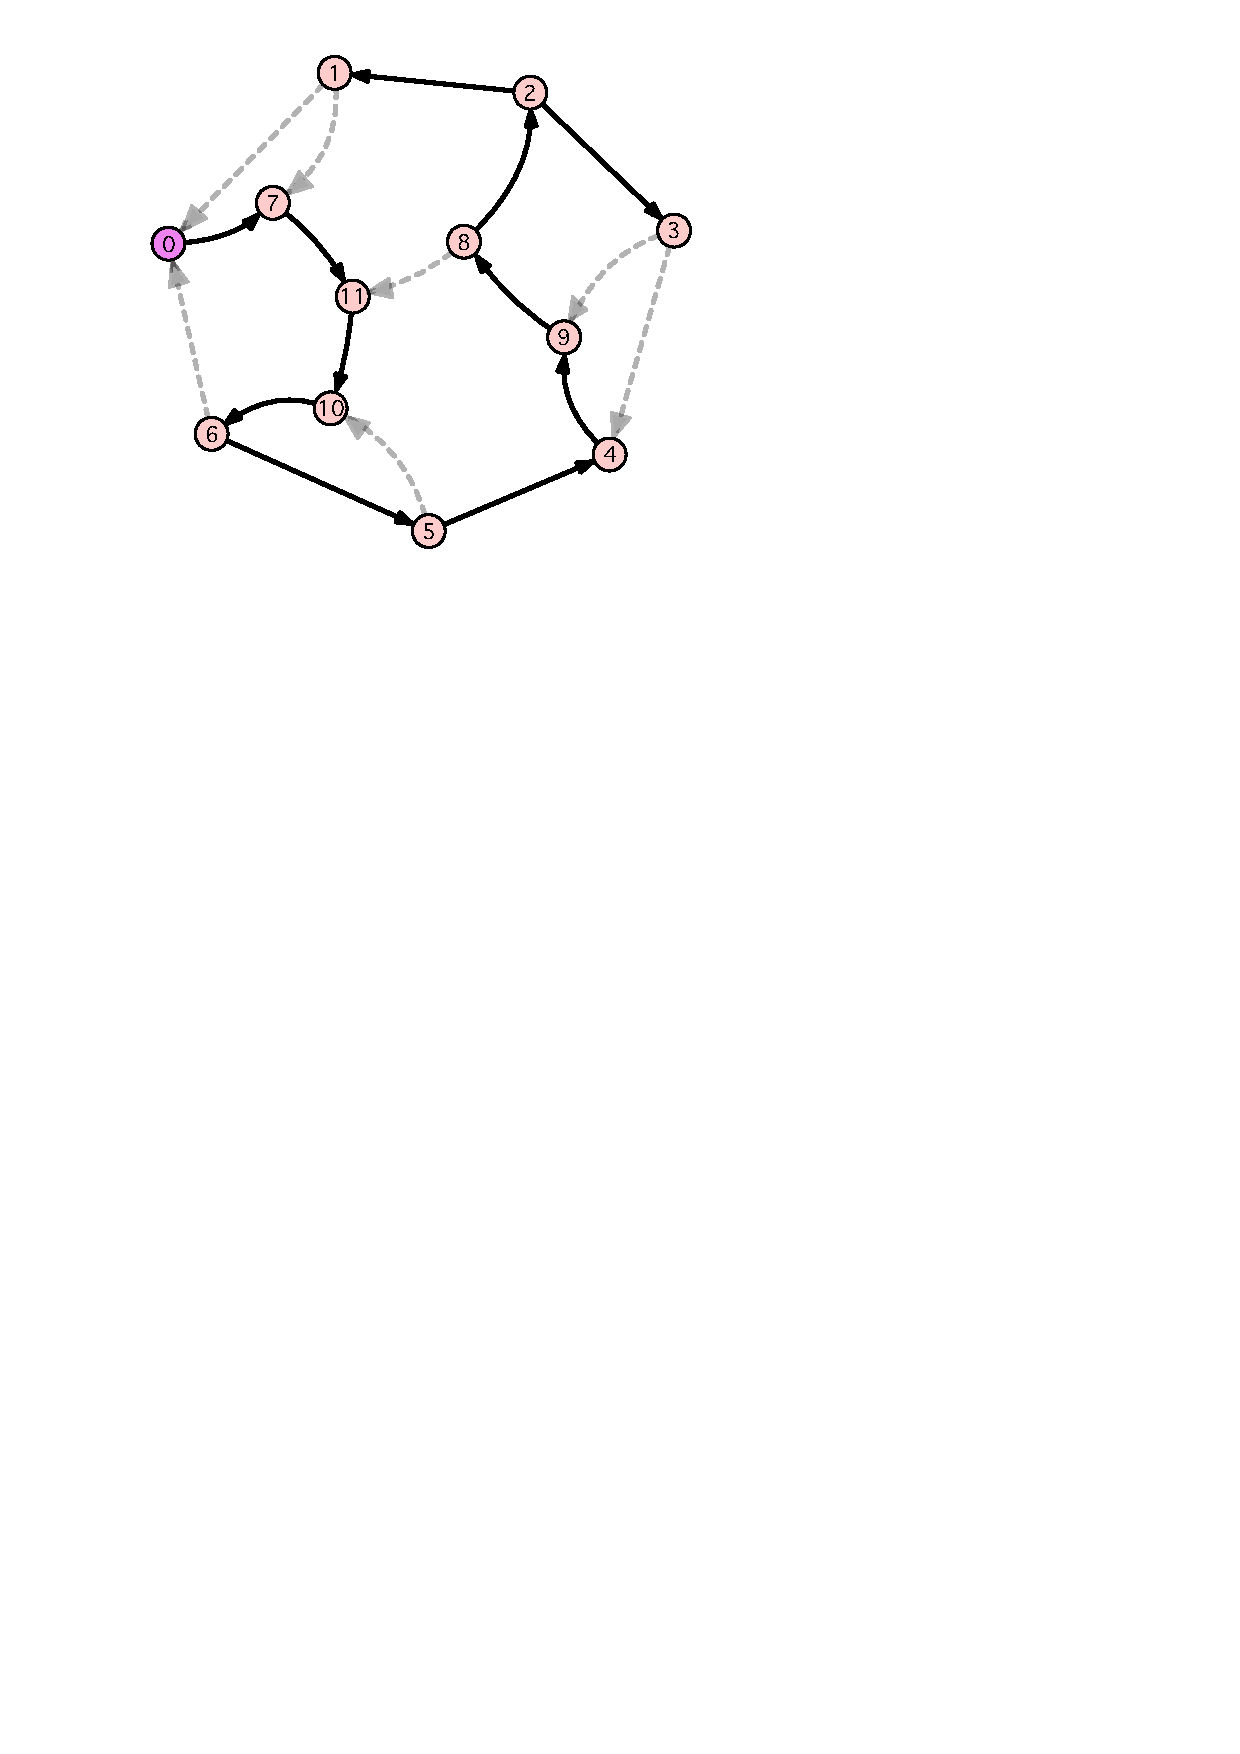
\includegraphics[width=0.24\textwidth]{figures/dfs_frucht2.pdf}
{\small フルフトグラフの\\深さ優先探索木の例}
%\label{fig:frucht_dfs_tree}
\end{figure}
\end{paracol}



\paragraph{深さ優先探索の基本コード}
下記の python コードは深さ優先探索の基本的な例である。
入力としてグラフ{\tt G}と根{\tt root}が与えられたとき、
{\tt G}において{\tt root}から到達可能な連結成分内の木辺と補木辺を表示する。
%木辺は未訪問の頂点の発見に貢献した辺で、それ以外は補木辺という。
%木辺という名称は、
%深さ優先探索の結果得られる木辺集合が誘導する部分グラフが
%対象グラフの全域木になっていることに由来する。
%補木辺は木辺集合の補集合に属すことから採っている。

\begin{lstlisting}[language=Python, caption=深さ優先探索の基本形,label=lst:dfs]
def dfs(G, root):
    stack, dfs_height = [(root, x) for x in G.neighbors(root)], {x: -1 for x in G}
    dfs_height[root] = 0
    while stack:
        parent, child = stack.pop()
        if dfs_height[child] < 0:
            stack += [(child, x) for x in G.neighbors(child) if x is not parent]
            dfs_height[child] = dfs_height[parent] + 1
            print((parent, child), ' is a tree edge')
        else:
            if dfs_height[parent] > dfs_height[child]:
                print((parent, child), ' is a back edge')
\end{lstlisting}%
%
\paragraph{コードの簡単な解説}
このコードでは、訪問すべき頂点対を管理する
データ構造としてスタック{\tt stack}を用いている(第2行)。
頂点対を対象とする理由は、
木辺と補木辺の組合せ構造がグラフの構造的性質を分析する一助となるからである。


また、訪問していない頂点を識別するために根からの距離を保持する連想配列
{\tt dfs\_height}を用いている(第2行)。
初期値を$-1$として、第6行目のように${\tt dfs\_height[child]} < 0$で
具体的に訪問していない頂点かどうかを判定する。
この判定が真となるなら{\tt (parent, child)}の頂点対は木辺であり、
偽なら終点{\tt child}の方が始点{\tt parent}より根に近いという条件付きで
補木辺と判定する(第11行)。

第6-9行は木辺に対する処理である。
つまり新たに未訪問の頂点$v$を発見したことを意味する。
このとき$v$と隣接する頂点のペアを作ってスタックに載せていく。
第5行目のスタックから頂点対{\tt (parent, child)}を取り出す処理は、
グラフ上では頂点{\tt parent}に遷移したことを意味する。

\paragraph{計算時間}
\lstrefname\ref{lst:dfs}の計算量は連結グラフを対象とするなら$O(m)$となる。
$m$は辺の個数。
これは、どの辺もスタックに追加される回数は1回、
取り除かれる回数も1回であることから測られる。
それ以外の隣接頂点リストの取得{\tt G.neighbors}、
スタックへの追加{\tt append}や削除{\tt pop}、
および連想配列の参照と更新{\tt dfs\_height[child]}は
単位時間で処理できるものとする。
%計算量に$n$が付記されているのは、$n < m$ のような非連結なグラフで、
%第7行目のスタック更新の際、結果として新たに追加する辺がない場合を考慮している。




%ここで、深さ優先探索木における半順序$\preceq$を定義する。



\paragraph{バックトラッキング}
深さ優先探索におけるバックトラックは、
子孫の部分木内のすべての頂点を訪問し終えた段階で行う処理工程をいう。
\lstrefname\ref{lst:dfs}はバックトラックを省略しているが、
下記の python コードのようにジェネレータ({\tt iter})を用いることで
バックトラックを明示的に備えることができる。
\lstrefname\ref{lst:dfs}との変更箇所を黄緑でハイライトしている。
\begin{lstlisting}[language=Python, caption=バックトラック付き深さ優先探索,
                   label=lst:dfs_back_track,escapechar=!]
def dfs_with_back_tracking(G, root):
    stack, dfs_height = [(root, !\hl{\mbox{\textcolor{magenta}{iter}}(G.neighbors(root)))}!], {x: -1 for x in G}
    dfs_height[root] = 0
    while stack:
        !\hl{parent, children = stack[-1]}!
        !\hl{\mbox{\textcolor{magenta}{try}}:}!
            !\hl{child = next(children)}!
            if dfs_height[child] < 0:
                !\hl{nbr = [x \mbox{\textcolor{magenta}{for}} x \mbox{\textcolor{magenta}{in}} G.neighbors(child) \mbox{\textcolor{magenta}{if}} x \mbox{\textcolor{magenta}{is not}} parent]}!
                !\hl{stack.append((child, \mbox{\textcolor{magenta}{iter}}(nbr)))}!
                dfs_height[child] = dfs_height[parent] + 1
                print((parent, child), ' is a tree edge')
            else:
                if dfs_height[parent] > dfs_height[child]:
                    print((parent, child), ' is a back edge')
        !\hl{\mbox{\textcolor{magenta}{except}} StopIteration:}!
            !\hl{\mbox{\textcolor{magenta}{if}} stack:}!
                !\hl{\mbox{\textcolor{magenta}{print}}(\mbox{\textcolor{codepurple}{'back tracking at'}}, stack[-1][0])}!
            !\hl{stack.pop()}!
\end{lstlisting}



%\vspace*{-0.7\intextsep}
\setcolumnwidth{0.6\textwidth, 0.4\textwidth}
\begin{paracol}{2}

%
\paragraph{コードの簡単な解説}
スタックが扱うデータ形式が異なるだけで基本的な仕組みは変わらない。
隣接頂点を直接スタックに持たせるのではなく、
隣接頂点の集合をジネレータ{\tt children}で扱う。

スタックの先頭が{\tt (parent, children)}のとき、
訪れるべき頂点は
{\tt next(children)}とすることで順次呼び出すことができる。
頂点{\tt parent}のすべての隣接頂点を訪れたら{\tt next}は
例外{\tt StopIteration}を生成する。
この例外を第16行目で受け取り、
第17行以降でバックトラック処理を記述することができる。


\switchcolumn
\begin{figure}[ht]
\centering
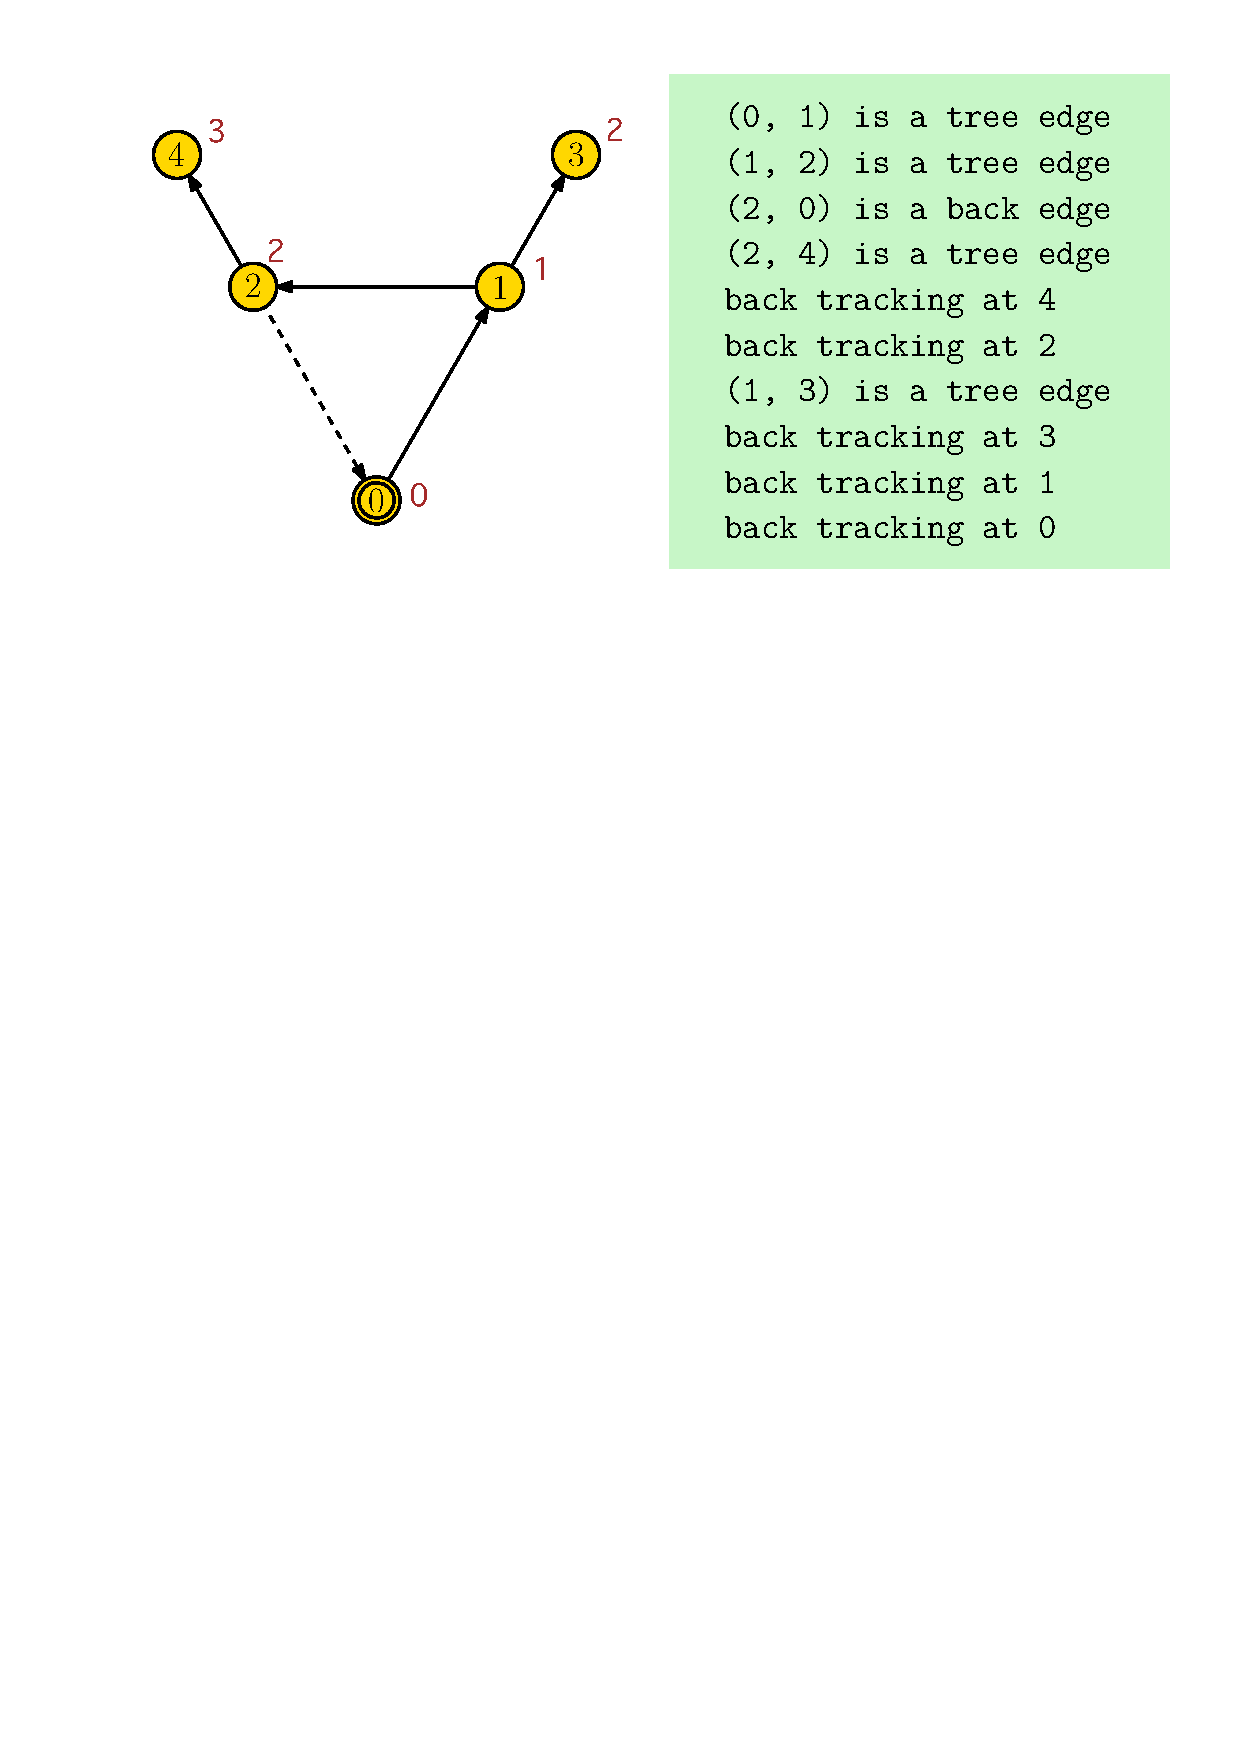
\includegraphics[width=0.39\textwidth]{figures/dfs_bull.pdf}
\end{figure}
\end{paracol}

\vspace*{-0.5\intextsep}
右図は雄牛グラフに対して頂点$0$を根として深さ優先探索を実行した例である。
実線矢印は木辺で破線矢印は補木辺。添字は深さ優先探索木における根までのパスの長さを表す。
また\lstrefname\ref{lst:dfs_back_track}の実行結果も緑の枠内に示している。







\subsection{深さ優先探索木の性質}


%\vspace{-1\intextsep}
\paragraph{深さ優先探索木上の高さと半順序}
各頂点$v$に関して深さ優先探索木${\mathcal T}$における高さ$h(v)$を
根から$v$までの${\mathcal T}$上の経路の長さとする。
${\mathcal T}$は木なのでどの二頂点間にも唯一の経路が存在する。
%\figurename\ref{fig:dfs_tree_icosahedral}では頂点$0$の高さは根なので$h(0)=0$。
上図の雄牛グラフの深さ優先探索木の例では頂点$0$の高さは根なので$h(0)=0$。
頂点$2$は根と隣接しているが${\mathcal T}$上の経路を考えるので$h(2)=2$。


\setcolumnwidth{0.8\textwidth, 0.2\textwidth}
\begin{paracol}{2}

任意の二頂点$x, y \in V$に関して${\mathcal T}$上の半順序$\preceq$を定義する。
$x \preceq y$で$x$が根から$y$までのパスに含まれることを表す。
反射律、反対称律、推移律を満たすことは容易に確認できる。
%半順序なので、\figurename\ref{fig:dfs_tree_icosahedral}の頂点$1$と頂点$3$のように
半順序なので右図の頂点$u$と頂点$v$のように
比較不能な頂点対が存在することを許す。



\paragraph{先祖と子孫}
この半順序関係に従って先祖と子孫の関係が定義できる。
$x \prec y$なら$x$は$y$の先祖。
$x \succ y$なら$x$は$y$の子孫。
${\mathcal T}_v$で
頂点$v$を根とし$v$と$v$の子孫から誘導される${\mathcal T}$の部分木を表す。
また、ある頂点$v$に対して、$v$から出て行く木辺の集合を$\omega^+(v)$で表す。
同様に$\omega^-(v)$で$v$から出て行く補木辺の集合とする。
例えば右図でいうと木辺$(x, y)$に対して$\omega^+(y)=\{(y, u), (y, v), (y, w)\}$であり、
$\omega^-(y)=\{(y, a), (y, b)\}$である。



\switchcolumn
\vspace{.5\intextsep}
\centering
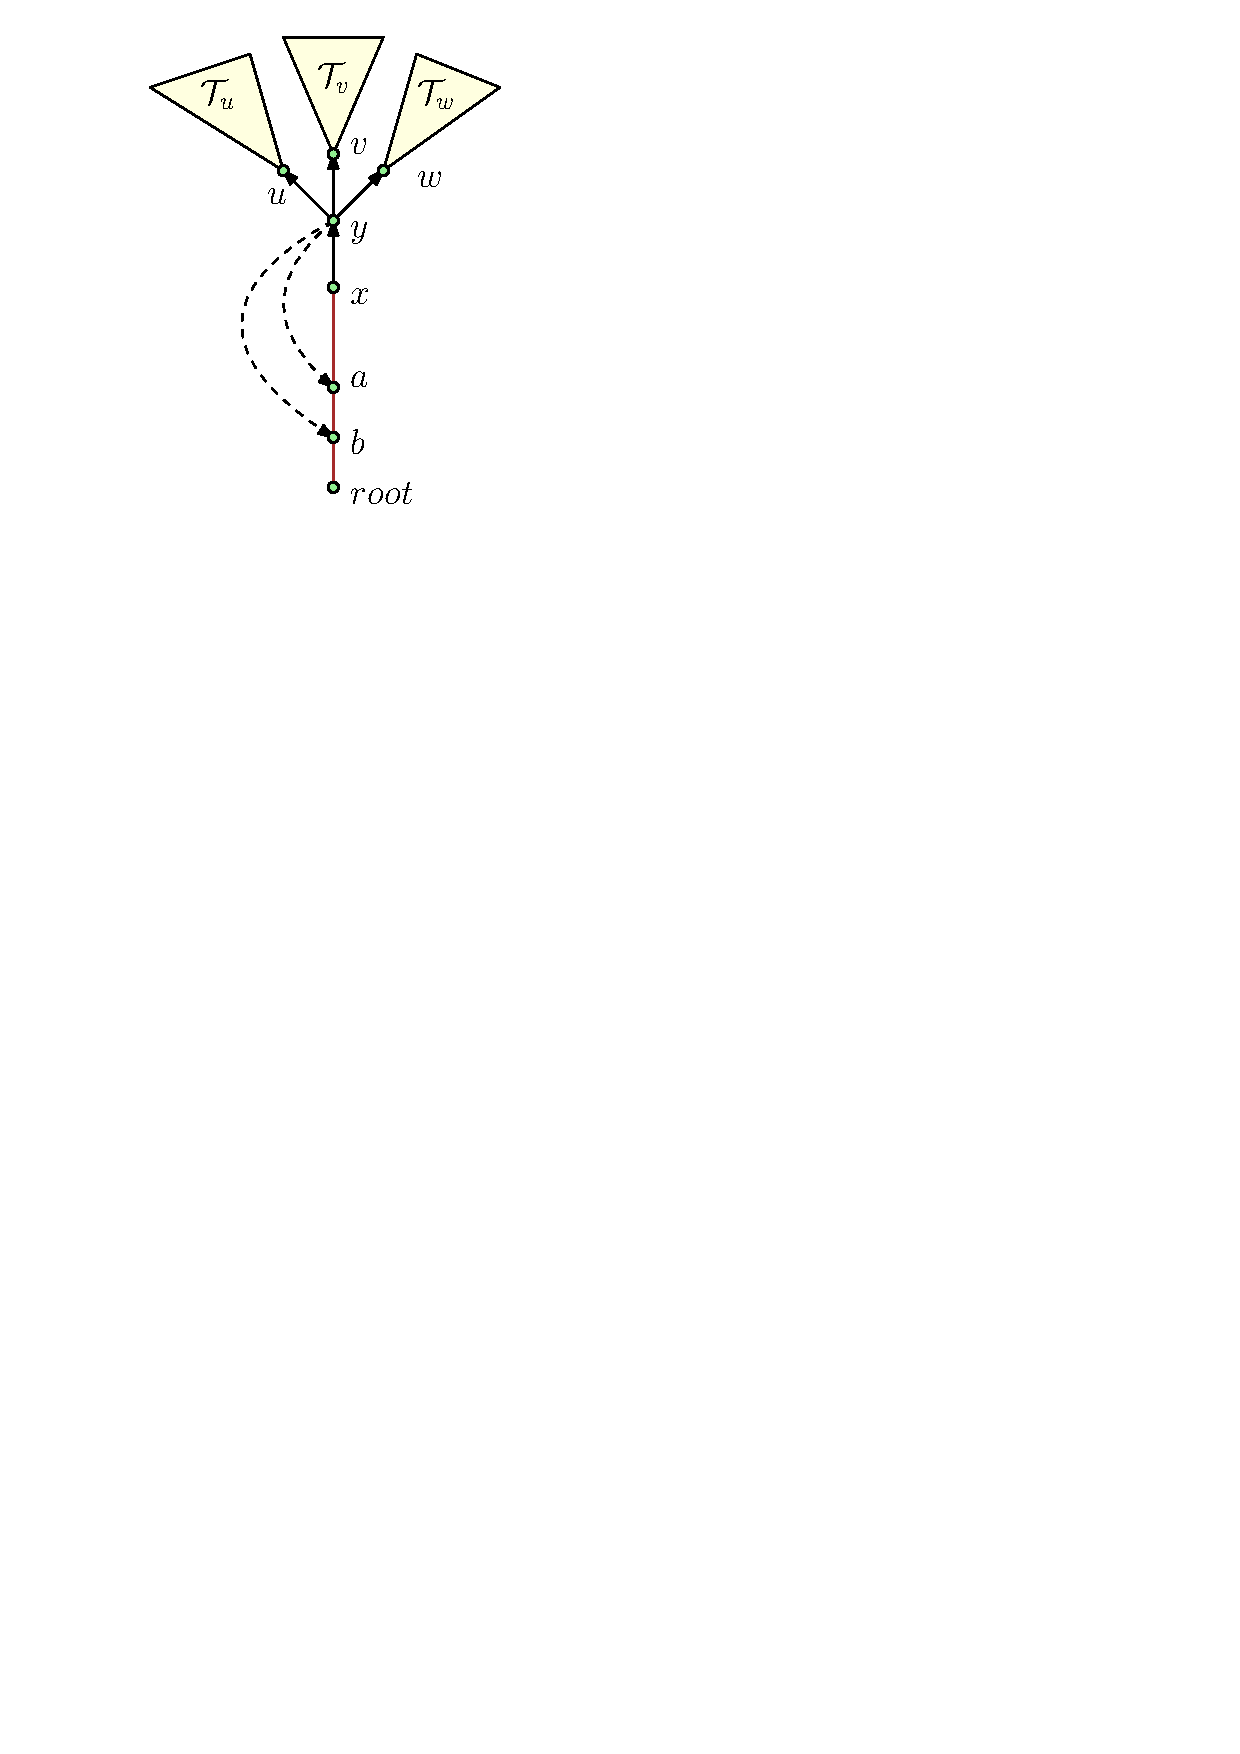
\includegraphics[width=0.18\textwidth]{figures/omegas.pdf}
\end{paracol}




%\vspace*{-0.7\intextsep}
\setcolumnwidth{0.75\textwidth, 0.25\textwidth}
\begin{paracol}{2}

\paragraph{深さ優先探索順序}
深さ優先探索に基づく頂点の遷移順序を定式化する。
$G=(V, E)$を$n$頂点の連結グラフとする。
$\sigma=(v_1, \ldots, v_n)$を$V$上の任意の置換とし、
$\sigma_i$で$i$番目までの部分列を表す。
頂点$v \in V \setminus \sigma_i$に関して
$\nu_{\sigma_i}(v)$で$\sigma_i$内に存在する$v$の隣接頂点の最後方の位置を表す。
$\sigma_i$内に隣接頂点が存在しない場合は$\nu_{\sigma_i}(v)=0$。
このとき次の条件を満たす$\sigma$を深さ優先探索順序という。
すべての$1 < i \leq n$に関して、
$\nu_{\sigma_{i-1}}(v_i) = \max\limits_{j=i,\ldots,n}\nu_{\sigma_{i-1}}(v_j)$。
%直感的には、$\sigma_i$を木と見做すと$\nu_{\sigma_i}(v)$は$v$と接続できる最近
%発見された頂点の$\sigma$上の位置となる。
%また、条件式で$\max$をとっているのは探索の最先端を意図する。

右図に対応する深さ優先順序として、例えば
$(0,11,10,9,8,7,2,6,5,4,3,1)$が得られる。
$i=5$のとき$\sigma_i=(0, 11,10,9,8)$であり、
$\nu_{\sigma_i}(7)=5$となる。%$\nu_{\sigma_i}(4)=3$。
頂点$7$は$\sigma_i$内のすべての頂点と隣接するが、
最後方の頂点$8$の位置$5$をとる。
頂点$6$は$\sigma_i$のどの頂点とも隣接しないので$\nu_{\sigma_i}(6)=0$。
また、$\sigma_i$に無い頂点$1,2,7$が$8$と隣接するので、
$\nu_{\sigma_{i}}(1) = 
\nu_{\sigma_{i}}(2) = 
\nu_{\sigma_{i}}(7) = 
\max\limits_{j=i,\ldots,n}\nu_{\sigma_{i}}(v_j)$。
このとき頂点$1, 2, 7$のいずれの選択も許されるが、
結果として得られる深さ優先探索木の構造は異なる可能性がある。

\switchcolumn
\vspace*{.5\intextsep}
%\begin{figure}[ht]
\centering
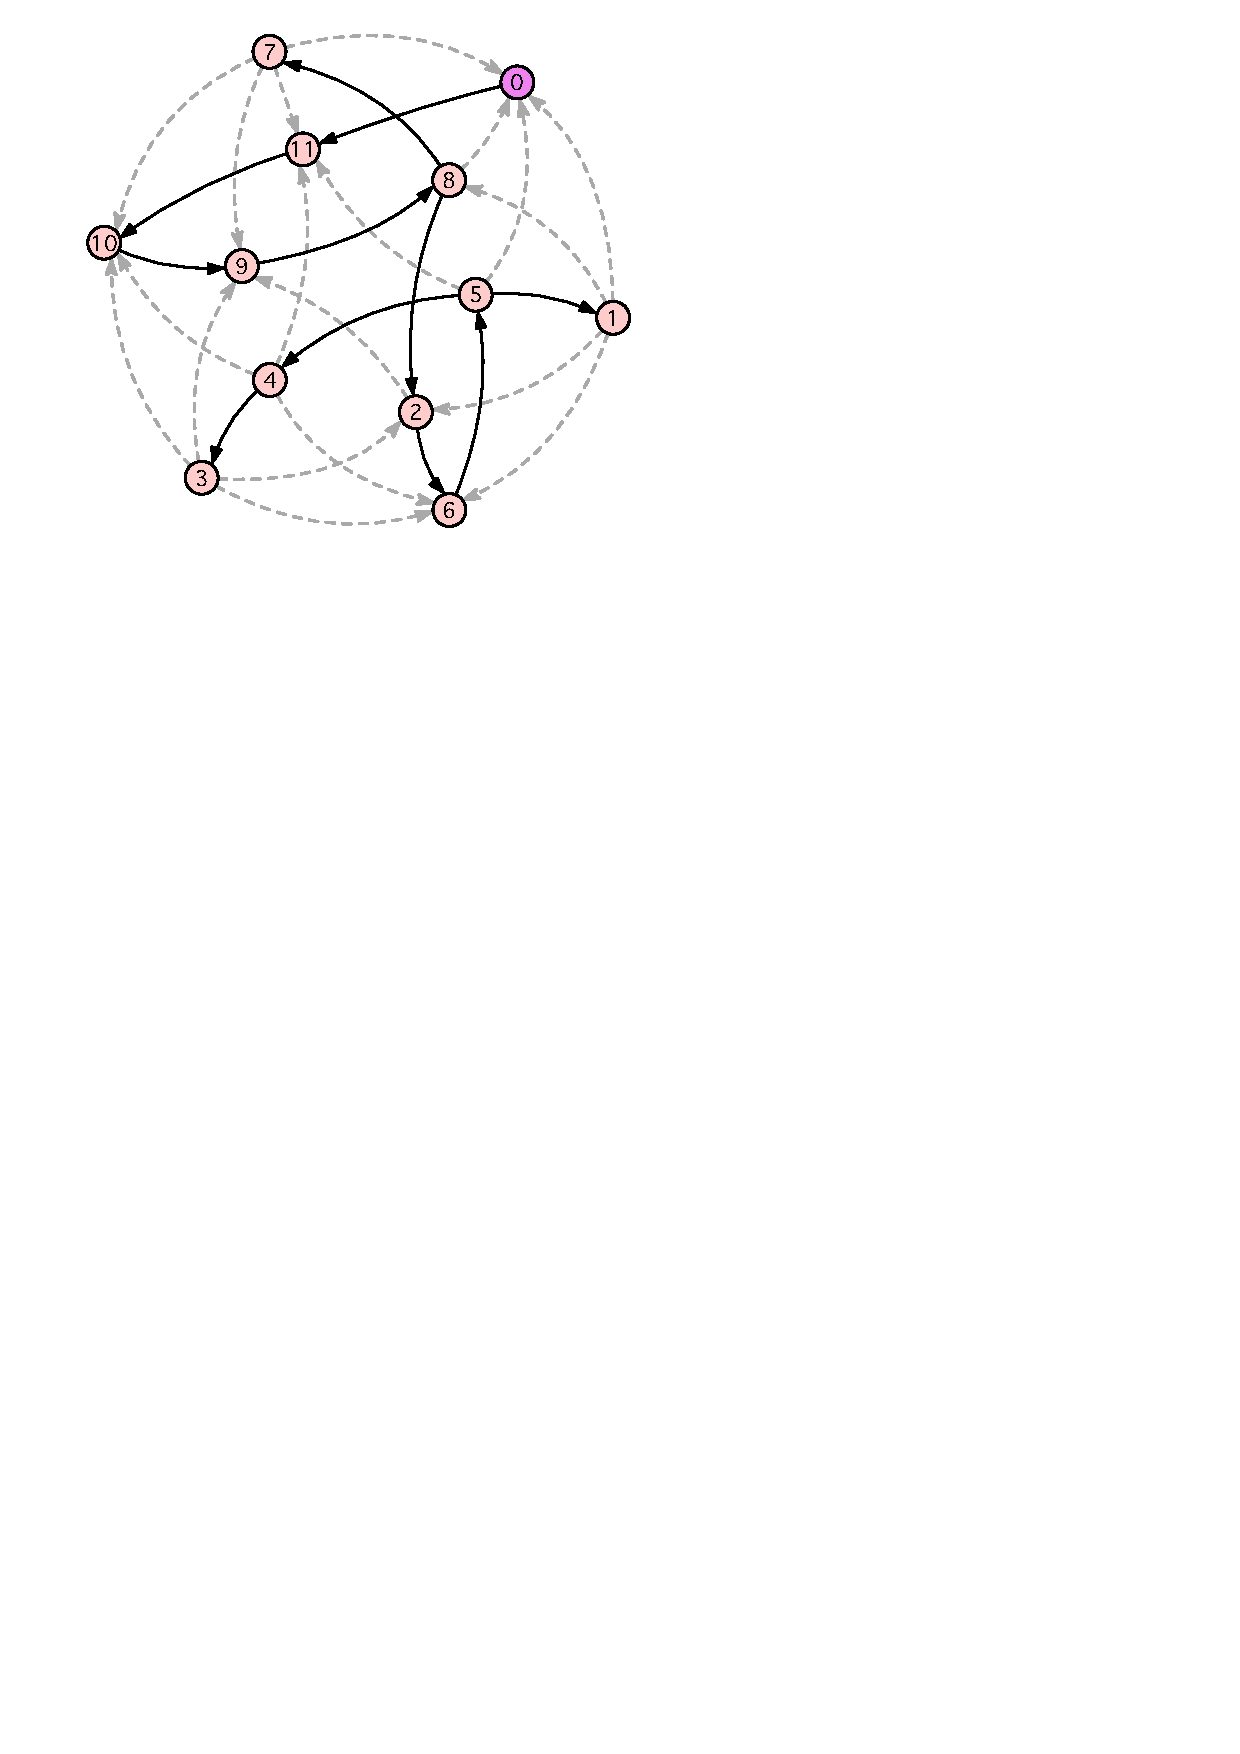
\includegraphics[width=0.23\textwidth]{figures/dfs_icosahedral.pdf}\\
{\small 十二面体グラフの\\深さ優先探索木}
%\caption{{\small 十二面体グラフの深さ優先探索木の例}}
%\label{fig:dfs_tree_icosahedral}
%\end{figure}
\end{paracol}


\begin{lemma}
\label{lemma:dfs_ordering}
連結グラフ$G=(V, E)$とその深さ優先探索木${\mathcal T}=(V, T)$において、
任意の補木辺$(x, y) \in E \setminus T$は$x\succeq y$を満たす。
\end{lemma}


\setcolumnwidth{0.8\textwidth, 0.2\textwidth}
\begin{paracol}{2}
\begin{proof}
$x \preceq y$なる補木辺$(x, y)$が存在すると仮定すると
深さ優先探索順序の条件式に矛盾する。

比較不能な頂点$x,y$間を接続する補木辺$(x,y)$が存在すると仮定する。
このとき$x\in {\mathcal T}_w$および$y \in {\mathcal T}_v$となる
頂点$u$および木辺対$(u, v), (u, w) \in \omega^+(u)$が存在する。
一般性を失うことなく、
${\mathcal T}$の深さ優先探索順序$\sigma$において$v$の方が$w$より前に現れるとする。
%$\omega^+(u)$の他の木辺の終点は$v$と$w$の間には現れないとする。
%$\sigma$において${\mathcal T}_v$の頂点の方が
%${\mathcal T}_w$の頂点より先に現れる。
%このとき$x$は$y$より先に発見されているので、
%$x, y$はそれぞれ${\mathcal T}_v, {\mathcal T}_w$の頂点である。
$k$を${\mathcal T}_v$の頂点の個数$-1$とし$\sigma$における$v$の位置を$i$とすると
$\sigma_{i+k}=w$となる。
また、${\mathcal T}_w$ の$w$を除く任意の頂点$x'$は$\nu_{\sigma_{i+k}}(x') = 0$。
しかし$x$と$y$は互いに隣接するので
$\nu_{\sigma_{i+k}}(w) < \nu_{\sigma_{i+k}}(x)$であり、
%深さ優先探索順序の条件式の下で
$x$は$w$より先に発見されなければならない。
帰納的にこれは$(u, w)$が木辺であることに矛盾する。
\end{proof}

\switchcolumn
\vspace{1.\intextsep}
\centering
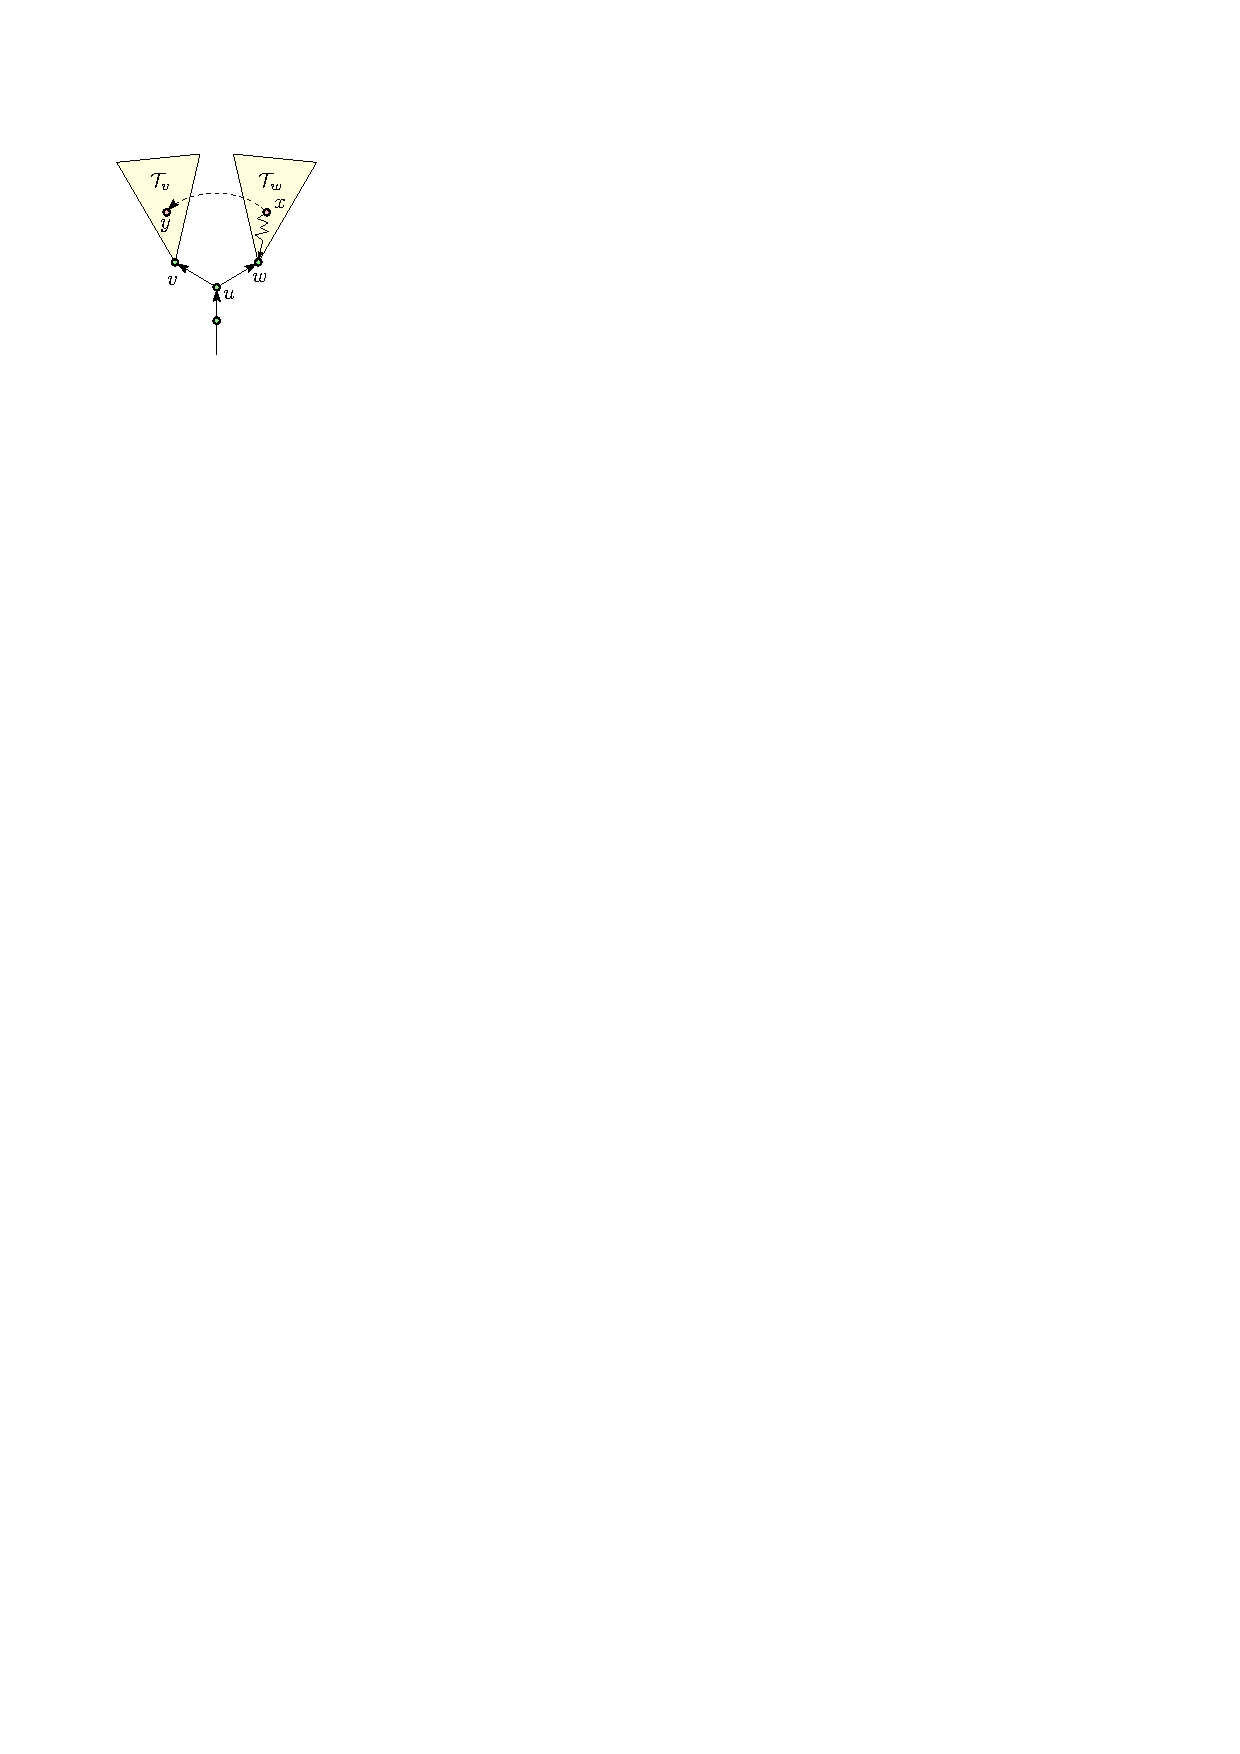
\includegraphics[width=0.19\textwidth]{figures/dfs_ordering2.pdf}
\end{paracol}

%\vspace{-0.5\intextsep}

\paragraph{補木辺の初等閉路}
任意の補木辺$e=(u, v)$は一意に定まる閉路を持つ。
つまり、$v$から$u$への木辺の系列に$e$を結合して得られる有向閉路である。
これを$e$の初等閉路と呼ぶ。
初等閉路の一意性は、
\cref{lemma:dfs_ordering}%深さ優先探索順序の条件式、
および深さ優先探索木${\mathcal T}$上の経路の一意性から導ける。



\setcolumnwidth{0.8\textwidth, 0.2\textwidth}
\begin{paracol}{2}
\paragraph{木辺のフリンジ}
%\cref{lemma:ignoring_back_edges}は、
\cref{lemma:dfs_ordering}により極小な部分問題を
定義づける補木辺の集まりであるフリンジを導入することができる。
深さ優先探索のバックトラックで$T \setminus E$内の探索範囲を限定し、
禁止構造の発見に貢献する補木辺とそれ以外とを区別する。
%注意を払わないといけない補木辺を区別する役割も持つ。


\begin{definition}
連結なグラフ$G=(V, E)$とその深さ優先探索木${\mathcal T}=(V, T)$が与えられたとき、
ある木辺$e = (x, y) \in T$のフリンジを次のように定義する。
\[
\fringe(e) = \{(u, v) \in E \setminus T ~|~ u \succeq y ~\mathrm{and}~ v \preceq x\}.
\]
\end{definition}


\switchcolumn
\vspace{.5\intextsep}
\centering
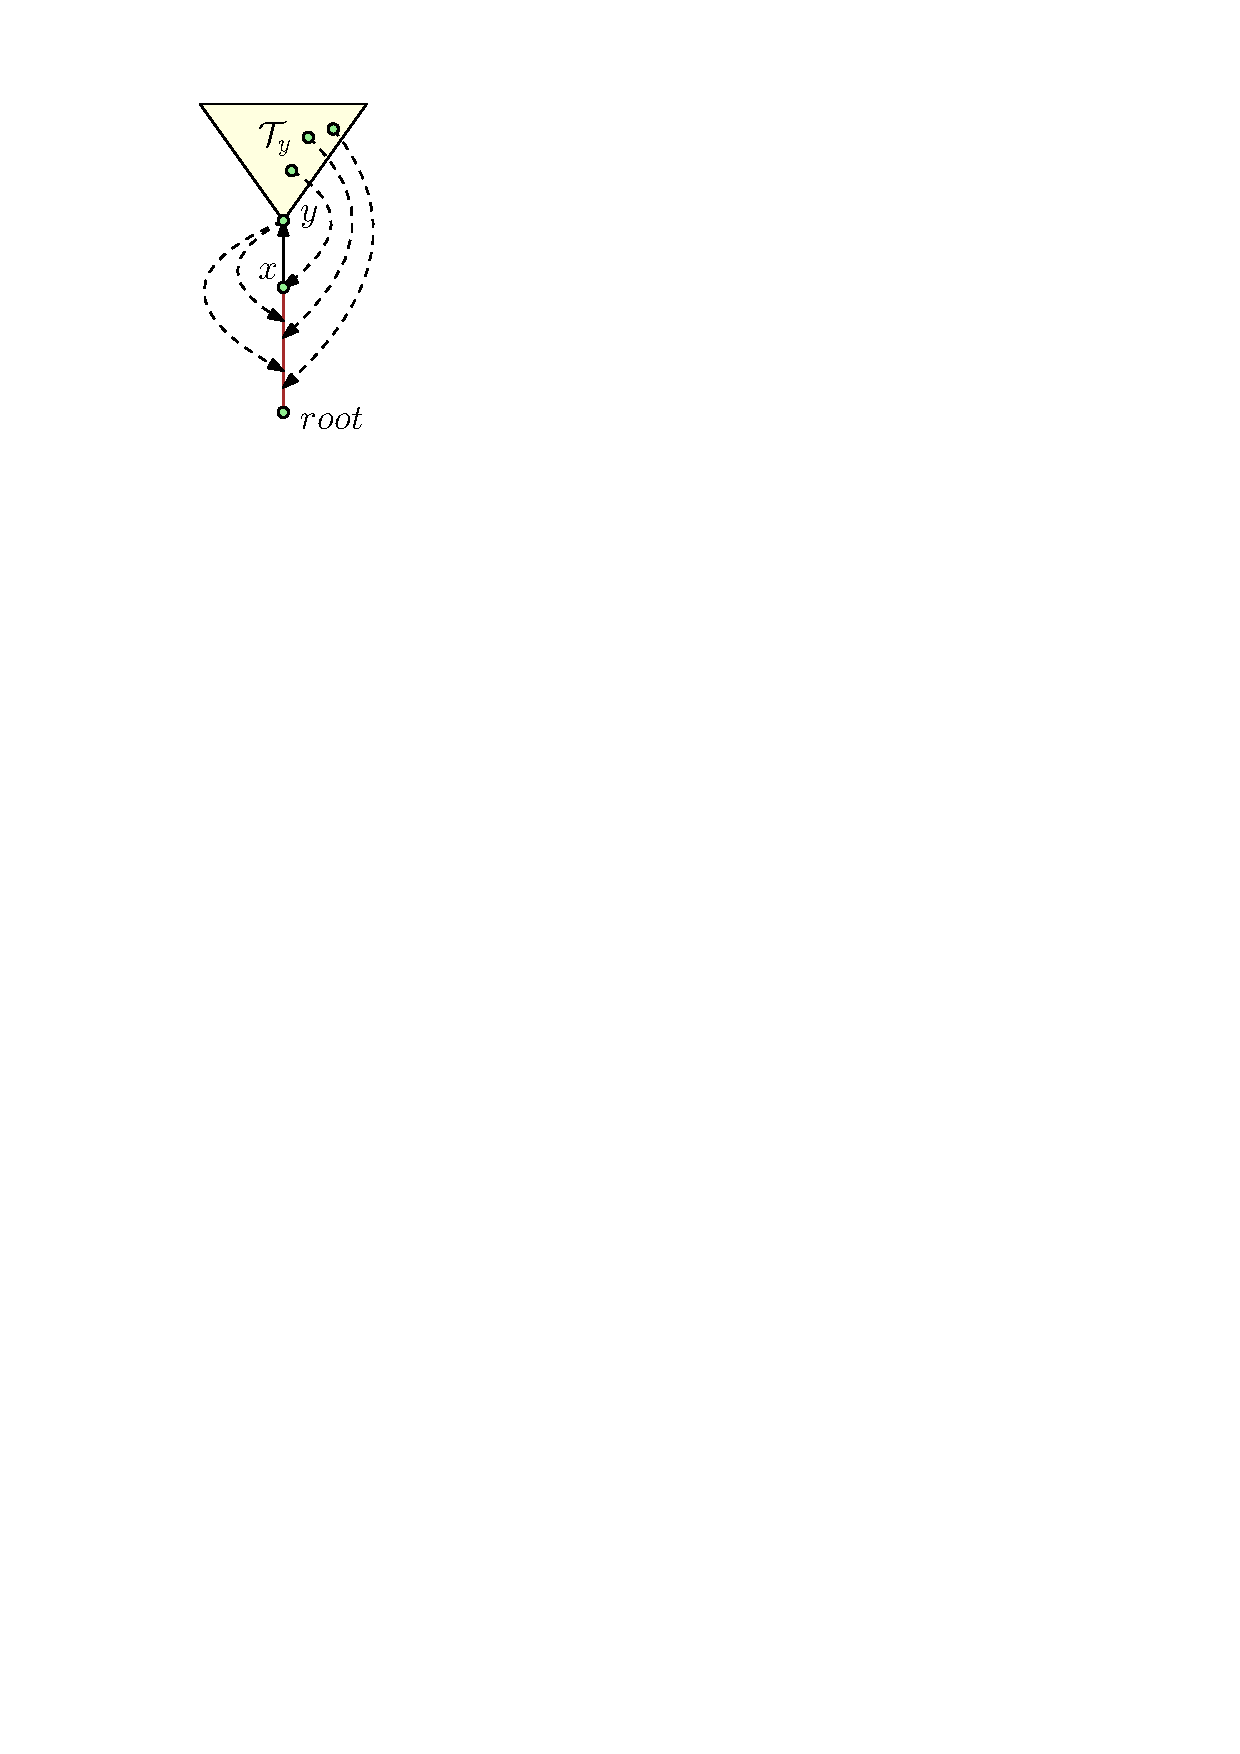
\includegraphics[width=0.1\textwidth]{figures/fringe_image1.pdf}
\end{paracol}

フリンジは対応する木辺$e=(x, y)$の${\mathcal T}_y$に始点を持ち
$y$の先祖に接続する補木辺の集まりである。
木辺$(x, y)$を基準に禁止構造の有無を調べる解法設計においては
$\fringe(e)$に限定できるかをきちんと考察する必要がある。
始点と終点がともに${\mathcal T}_y$にある補木辺の集合
$T_{\succeq y}=\{(u, v) \in E \setminus T ~|~ y \preceq v\}$が
比較対象外にできれば効率は大きく変わる。

%ただし、平面性判定においては補木辺の終点の高さだけでなく視点の高さも禁止構造に
%関係するので判定で用いる位相構造の不変条件には注意が必要である。



\begin{comment}
\begin{lemma}
\label{lemma:ignoring_back_edges}
%グラフ$G=(V, E)$およびその深さ優先探索木${\mathcal T}=(V, T)$に関して、
ある頂点$v$の子孫の部分木${\mathcal T}_v$の辺集合$T_v$および
$T_{\geq h(v)}$が誘導する
部分グラフ$G[T_v \cup T_{\geq h(v)}]$が禁止構造を含まないなら
%すなわち平面的なら
$v$の先祖の判定において$T_{\geq h(v)}$内のすべての補木辺は
比較の対象外として良い。
ただし、位相構造の制約は保持される場合がある。
\end{lemma}

\begin{proof}
\cref{lemma:dfs_ordering}より
$v_1, v_2 \in \omega^+(v)$に関して、
${\mathcal T}_{v_1},~{\mathcal T}_{v_2}$は互いに点素であり辺素である。
禁止構造が存在するとすれば
$\bigcup\limits_{e_i \in \hat{o}(v)} \fringe(e_i) \setminus T_{\geq h(v)}$
内の補木辺の組合せに拠る。
ただし$\hat{o}(v) = \{(v, v_i) ~|~ v_i \in \omega^+(v)\}$。
\end{proof}
\end{comment}


%一意性は深さ優先探索順序の条件式、および${\mathcal T}$上のパスの一意性から導ける。
%一意性は



%\begin{corollary}[子孫の部分木の包含関係と排他性]
%反順序$\succeq$の推移律から$x \preceq y$なら
%${\mathcal T}_y \subseteq {\mathcal T}_x$が成り立つ。
%$(y, u)$と$(y, v)$が始点$y$を共有する木辺であるなら
%${\mathcal T}_u \cap {\mathcal T}_v = \varnothing$が成り立つ。
%これも推移律から${\mathcal T}_u$および${\mathcal T}_v$それぞれの
%任意の部分木間にも排他性が成り立つ。
%\end{corollary}
%半順序$\preceq$は深さ優先探索木に対して重要な特徴付けを与える。
%まず、すべての木辺$(x, y)$は$x \prec y$であり、
%すべての補木辺$(x, y)$は$x \succ y$。
%補木辺が比較不能な頂点どうしを接続しないことは
%深さ優先探索順序の条件式が保証する。









%%%%%%%%%%%%%%%%%%%%%%%%%%%%%%%%%%%%%%%%%%%%%%%%%%%%%%%%%%%%%%%%%%%%%%%%%%%%%%%%%%%%
\subsection{グラフの\texorpdfstring{$2$}-辺連結性}
ここでは深さ優先探索に基づきグラフの構造分析の応用として$2$-辺連結性を判定する
問題を考察する。
特に、\cref{lemma:dfs_ordering}および%\cref{lemma:ignoring_back_edges}
フリンジが定義する極小な部分問題の重要性を確認したい。
グラフの$2$-辺連結性は任意の辺を削除しても連結性を損なわない性質をいう。
別の言い方をすると禁止構造としての橋を持たないグラフである。


%$2$-辺連結性判定のアルゴリズムを記述する前に基本的な事実を確認する。


\begin{lemma}\label{lemma:bridge_is_tree_edge}
橋は木辺。
\end{lemma}
\begin{proof}
補木辺となる橋が存在すると初等閉路の$2$-辺連結性に矛盾。
\end{proof}

\begin{lemma}\label{lemma:no_bridge_has_illegal_cotree_edges}
木辺$e=(x, y)$が橋である必要十分条件は、
%$u \succeq y$および$v \preceq x$を端点とする補木辺$(u, v)$を持たないこと。
$\fringe(e)=\varnothing$であること。
\end{lemma}
\begin{proof}
必要性は背理法で。
主張の前提を満たす補木辺$f\in\fringe(e)$が存在すると仮定すると$f$の初等閉路は$e$を含む。
%\cref{lemma:bridge_is_tree_edge}より、$e$は$f$初等閉路の構成要素なので矛盾。
十分性は演繹的に。
${\mathcal T}_y$の頂点を始点として持たない補木辺は初等閉路内に$e$を含まない。
終点を${\mathcal T}_y$内に持たない場合、
%深さ優先探索順序の条件式より
\cref{lemma:dfs_ordering}は
$y$が根から$x$までのパス上に存在することを保証する。
%同様に両端点を$x$の子孫に持つ補木辺の初等閉路も$e$を含まない。
%$x$の子孫を始点として$x$の子孫でも$y$の先祖でない頂点に接続する補木辺は、
%深さ優先探索の性質上存在しない。
\end{proof}

%\begin{corollary}\label{coro:not_bridge}
任意の補木辺$e=(x, y)$に関して、根から$x$への木辺の系列のうち
頂点$y$以降の各木辺は橋ではない。
従って$\fringe(e)$内の補木辺の終点の高さの最小値
$\min\limits_{(u, v)\in\fringe(e)} h(v)$を適切に管理すれば良い。

%\end{corollary}


\paragraph{$2$-辺連結性判定のpythonコード}
\cref{lemma:no_bridge_has_illegal_cotree_edges}%および
を踏まえると次のような python コードが得られる。
このコードは橋を見つけた時点で$2$-辺連結性を有さないと判定する。
また、\lstrefname\ref{lst:dfs_back_track}との変更箇所を黄緑でハイライトしている。
\begin{lstlisting}[language=Python, caption=$2$-辺連結性判定{\tt has\_bridge},
                   label=lst:dfs_2_edge_connectivity,escapechar=!]
def has_bridge(G, root):
    stack, dfs_height = [(root, iter(G.neighbors(root)))], {x: -1 for x in G}
    dfs_height[root] = 0
    !\hl{lowest = []}!
    while stack:
        parent, children = stack[-1]
        try:
            child = next(children)
            if dfs_height[child] < 0:
                nbr = [x for x in G.neighbors(child) if x is not parent]
                stack.append((child, iter(nbr)))
                dfs_height[child] = dfs_height[parent] + 1
                !\hl{lowest.append([])}!
            else:
                if dfs_height[parent] > dfs_height[child]:
                    !\hl{set\_lower(lowest[-1], dfs\_height[child])}!
        except StopIteration:
            !\hl{child, \_ = stack.pop()}!
            !\hl{\mbox{\textcolor{magenta}{if}} len(lowest) > 0:}!
                !\hl{\mbox{\textcolor{magenta}{if len}}(lowest[-1]) == 0:}!
                    !\hl{\mbox{\textcolor{magenta}{return}} (stack[-1][0], child)}!
                !\hl{prune(lowest, dfs\_height[stack[-1][0]])}!
\end{lstlisting}

\paragraph{コードの簡単な解説}
新たに配列の配列{\tt lowest}を導入し、各木辺$(x, y)$の終点の子孫${\mathcal T}_y$を始点とする
補木辺の終点の高さを管理する。厳密には最も根に近い終点の高さ、つまり高さの最小値を管理する。
橋の検出の場合{\tt lowest}は単純に整数の配列でも用途は足りるが、
後述の平面性判定では${\mathcal T}_y$内の頂点を始点とする複数の補木辺を管理することとなるため
配列の配列として定義している。


\begin{figure}[ht]
    \centering
    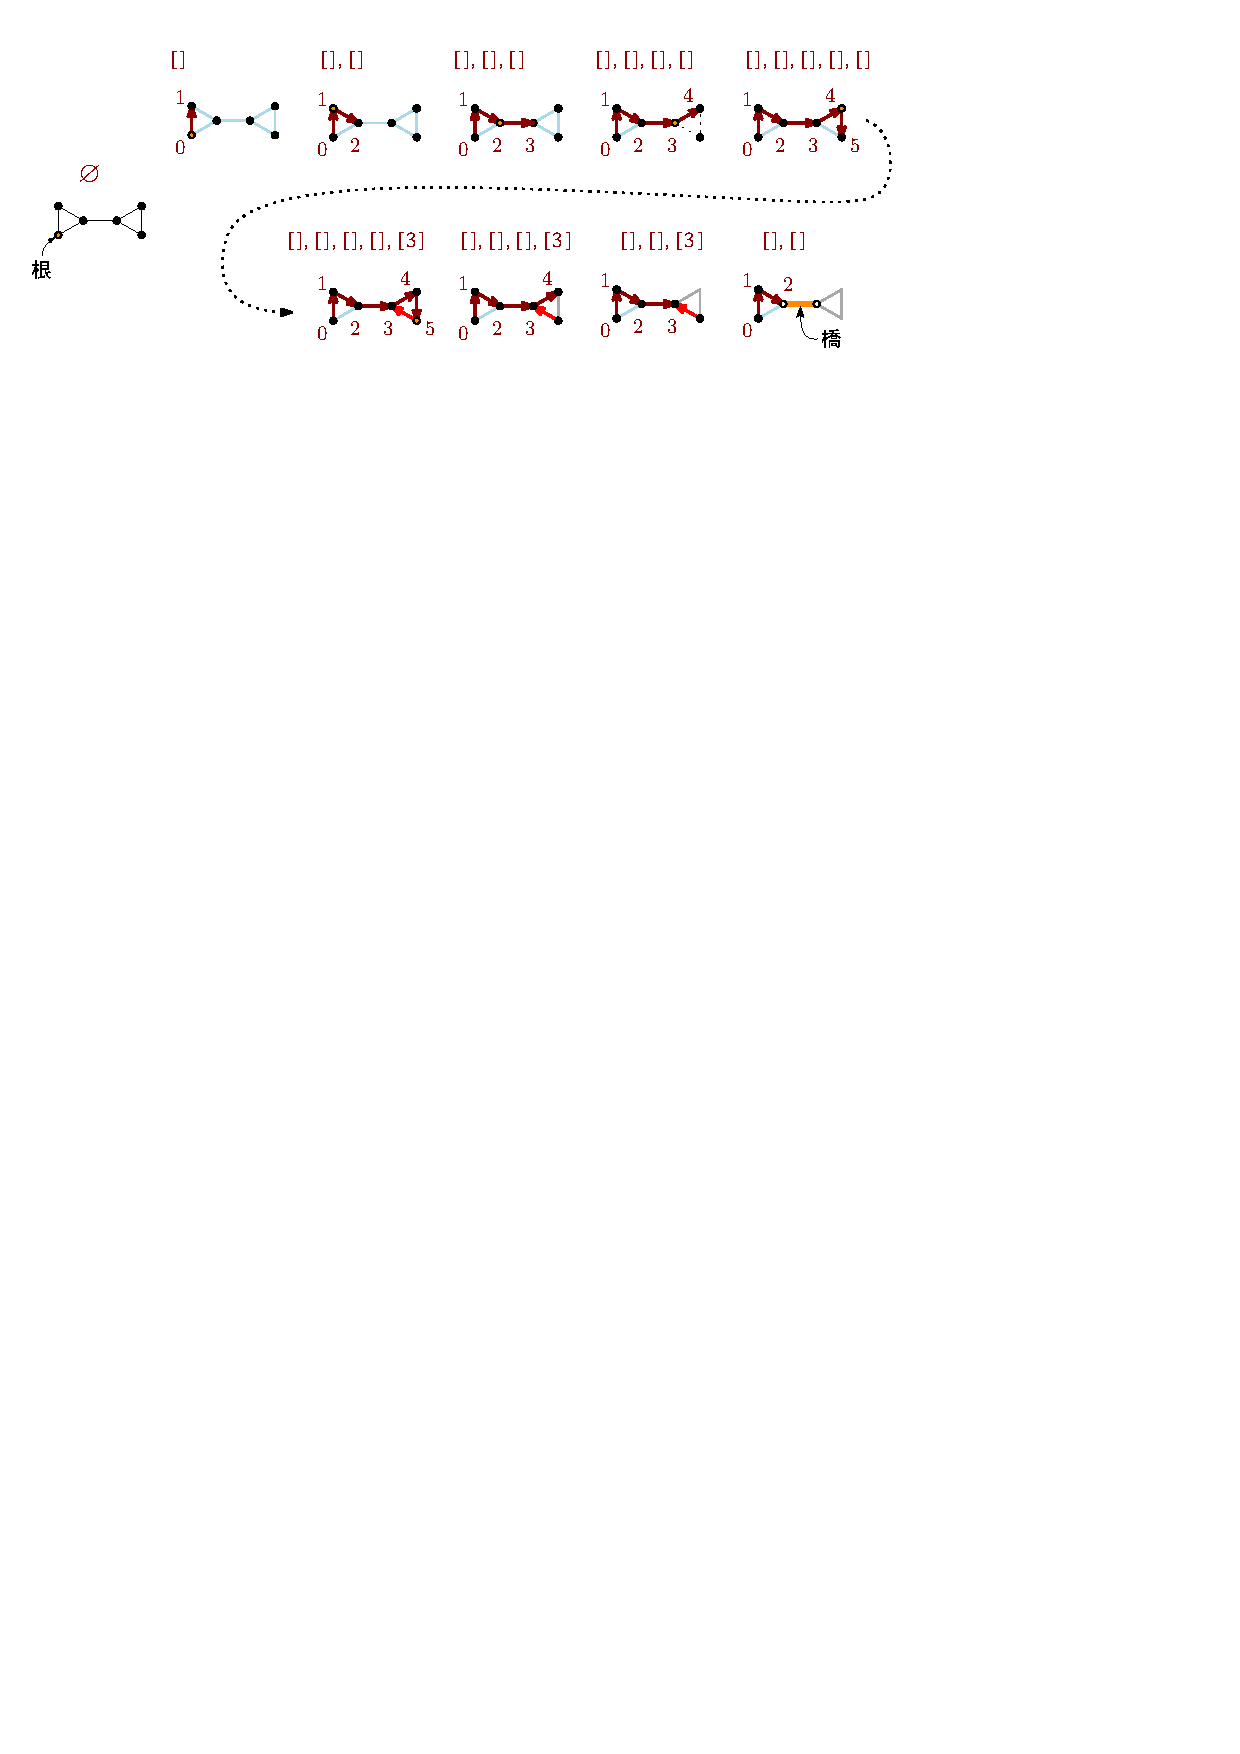
\includegraphics[width=0.95\textwidth]{figures/bridge_illust.pdf}
\end{figure}






探索の初期段階では補木辺は検出されないため空の配列が積み上がっていく(第13行)。
補木辺を見つけたらその終点の高さを{\tt lowest}の末尾の配列に追加する(第16行)。
関数{\tt set\_lower}は対象の配列が空でない場合小さい方を採用する。

橋の具体的な検出はバックトラックで行う。
{\tt lowest}の末尾が空の場合、\cref{lemma:no_bridge_has_illegal_cotree_edges}により
橋が存在すると判定する(第20-21行)。
橋でなかった場合、関数{\tt prune}を用いて先祖の木辺のために補木辺の情報を継承させる。
この際、木辺の終点の高さと{\tt lowest}の末尾の補木辺の終点の高さが等しい場合は継承せずに破棄する。




\lstrefname\ref{lst:dfs_2_edge_connectivity}は二つの
手続き{\tt set\_lower}と{\tt prue}を用いる。
{\tt set\_lower}はより根に近い補木辺の高さを設定する。
引数に{\tt pos}があるのは対象が現行の木辺の更新なのか、
先祖の木辺への更新なのかを切り替えられるよう策定している。
{\tt prune}は不要な補木辺の情報を取り除き、先祖の木辺へ情報を伝播する。
%いずれも簡潔なので解説は省略する。
%これは、\cref{lemma:no_bridge_has_illegal_cotree_edges}に従い
%以降の探索のバックトラックで対象となるいずれの木辺も
%その初等閉路に含まないことを意味する。

\begin{lstlisting}[language=Python, caption=set\_lower,
                   label=lst:set_lower]
def set_lower(pos, h):
    if len(pos) != 0:
        pos[0] = min(pos[0], h)
    else:
        pos.append(h)
\end{lstlisting}

\begin{lstlisting}[language=Python, caption=prune,
                   label=lst:prune_2_edge_connectivity]
def prune(lowest, over_height):
    h = lowest[-1].pop()
    lowest.pop()
    if h < over_height:
        set_lower(lowest[-1], h)
\end{lstlisting}

\paragraph{正当性と計算時間}
アルゴリズムの正当性は
\cref{lemma:no_bridge_has_illegal_cotree_edges}から導ける。
計算量は深さ優先探索と同程度の$O(|E|)$時間で抑えられる。
{\tt stack}の末尾の木辺$(x, y)$に対する最小値更新に係る計算量は、
{\tt set\_lower}を呼び出す回数であり、
頂点$y$から出て行く補木辺の個数に比例するので$O(|\omega^-(y)|)$。
バックトラック時のコストは
%不要な補木辺情報の破棄、および先祖の{\tt lowest}に継承するコスト、
{\tt set\_lower}および{\tt prune}いずれも高々一回呼出しなので$O(1)$となる。
まとめると対象の連結グラフ$G=(V, E)$と
その深さ優先探索木${\mathcal T} = (V, T)$に対して
$\sum\limits_{(x, y) \in T}O(|\omega^-(y)|)+
\sum\limits_{(x, y) \in T}O(1) = O(|E \setminus T|)+O(|T|)=O(|E|)$を得る。




%\subsection{フリンジのデータ構造}
%各木辺に付随するフリンジは平面性判定の極小単位を与える補木辺の部分集合である。
%平面性判定アルゴリズムは、
%各木辺のフリンジ内にクラトフスキー部分グラフの存在確認をそのサイズの線形時間で処理する。
%すべての木辺について調べてクラトフスキー部分グラフが確認できなければ
%対象グラフは平面的であると判定する。


\paragraph{まとめ}
橋でないことを保証するために、各木辺$(x, y)$に対して
$h(x)$と$y$の子孫の補木辺の終点の高さの最小値{\tt lowest}を対応づけ、
一つ一つ健全性を確認しながら進めていく。
バックトラックで子孫の{\tt lowest}を適切に継承し
所望の不変性を維持しつつ({\tt set\_lowest})、
不要な補木辺を破棄する({\tt prune})。
大事なことは監視対象である終点の高さの引き継ぎと適時開放。
これをバックトラック時に適切かつ効率良く処理する手順の設計がとても重要な観点である。

%また、深さ優先探索に基づく構造分析は、
%まず深さ優先探索木があって、木構造は禁止構造ではなく、
%補木辺や初等閉路の組合せによって誘発される禁止構造の特定に
%適するアプローチといえる。
